\documentclass[tikz,border=10pt]{standalone}
\begin{document}
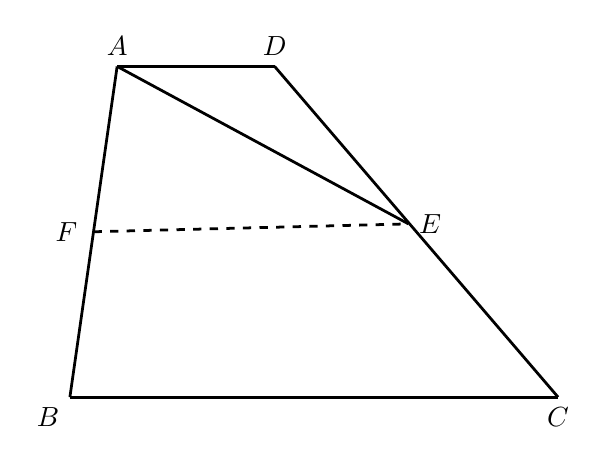
\begin{tikzpicture}[line width=1pt]
  \coordinate (A) at (0.6,4.6);
  \coordinate (D) at (2.6,4.6);
  \coordinate (B) at (0,0.4);
  \coordinate (C) at (6.2,0.4);
  \coordinate (E) at (4.3,2.6);
  \coordinate (F) at (0.3,2.5);

  \draw (A) -- (D);
  \draw (D) -- (C);
  \draw (C) -- (B);
  \draw (B) -- (A);
  \draw (A) -- (E);
  \draw[dashed] (F) -- (E);

  \node[above] at (A) {$A$};
  \node[above] at (D) {$D$};
  \node[below left] at (B) {$B$};
  \node[below] at (C) {$C$};
  \node[right] at (E) {$E$};
  \node[left=2pt] at (F) {$F$};
\end{tikzpicture}
\end{document}
